\documentclass{article}

% 导入中文宏包
\usepackage{ctex}
\usepackage{array}
\usepackage{caption}
\usepackage{hyperref}
% 设置页面边距
\usepackage{geometry}
\usepackage{graphicx}
\geometry{a4paper, left=2.5cm, right=2.5cm, top=3cm, bottom=3cm}

% 设置标题、作者和日期
\title{Shell和Vim学习}
\author{23020007160  张绍延}

\begin{document}

% 生成标题、作者和日期
\maketitle

% 心得报告正文
\section{实验目的}
本次课程主要讲授了Shell工具和脚本,用编辑器Vim进行数据整理。

\section{介绍}
\subsection{两大工具的优点}
1.Shell的优点:Shell脚本可以将多个命令组合在一起,自动执行重复性的任务,大大提高工作效率。
Shell可以很容易地调用其他编程语言(如Python、Perl等)编写的脚本或程序。

2.Vim有一个非常高效的编辑模型,熟练使用后可以大大提高文本编辑速度。Vim可以在命令行中直接
使用,非常适合在服务器或远程环境中进行文本编辑。
\section{练习内容}
\subsection{Shell学习例子10个}

1.echo "Hello, World!"用Shell打印hello world
echo 是一个在命令行界面(shell)中常用的命令,
它的主要作用是输出(显示)一段文本或者变量的值到标准输出

\noindent
\begin{minipage}{\linewidth}
  \centering
  % 插入图片
  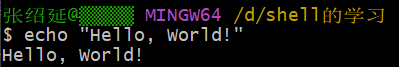
\includegraphics[width=0.5\linewidth]{shell1.png}
  % 图片标题
  \captionof{figure}{echo 用来显示文本或变量}
  \label{fig:example}
\end{minipage}


2.变量赋值以及变量的使用
\begin{verbatim}
    word="Hello, Git Bash!"
    echo $word
    #向word变量赋值,再通过echo $输出变量
 \end{verbatim}


\noindent
\begin{minipage}{\linewidth}
  \centering
  % 插入图片
  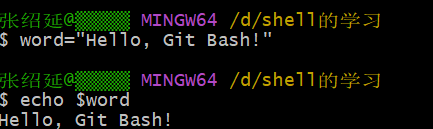
\includegraphics[width=0.5\linewidth]{shell2.png}
  % 图片标题
  \captionof{figure}{变量的赋值和使用}
  \label{fig:example}
\end{minipage}

3.条件语句的判断
 \begin{verbatim}
    if [ "$word" = "Hello, Git Bash!" ];then
      echo "Yes."
    else
      echo "No."
    fi
   #[]里是条件判断,then后面是条件正确的结果,else是条件错误的结果
   
 \end{verbatim}

\noindent
\begin{minipage}{\linewidth}
  \centering
  % 插入图片
  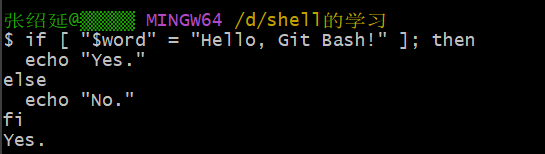
\includegraphics[width=0.5\linewidth]{shell3.png}
  % 图片标题
  \captionof{figure}{条件语句的判断}
  \label{fig:example}
\end{minipage}

4.循环的使用
\begin{verbatim}
    for i in {1..5}; do
     echo "number: $i"
    done
    #in {1..5} 指定了循环的范围。
  在这个例子中,{1..5} 是一个序列表达式,表示从1到5的数字序列,包括1和5。
  done是结束这个循环
\end{verbatim}

\noindent
\begin{minipage}{\linewidth}
 \centering
  % 插入图片
  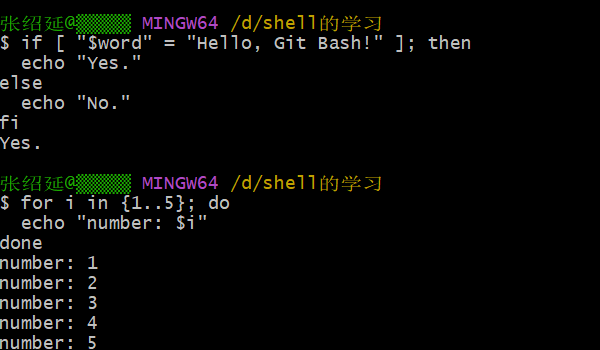
\includegraphics[width=0.5\linewidth]{shell4.png}
  % 图片标题
  \captionof{figure}{循环语句}
  \label{fig:example}
\end{minipage}



5.文件的创立与写入
\begin{verbatim}
    创建一个新文件
    touch example.txt
    
    写入内容到文件
    echo "This is an example file." > example.txt
    
    读取文件内容
    cat example.txt     
\end{verbatim}


\noindent
\begin{minipage}{\linewidth}
 \centering
  % 插入图片
  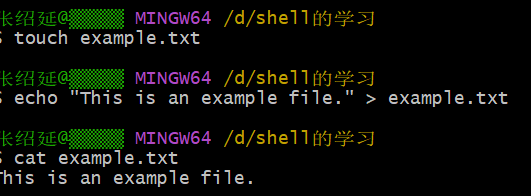
\includegraphics[width=0.5\linewidth]{shell5.png}
  % 图片标题
  \captionof{figure}{创建写入读取文件}
  \label{fig:example}
\end{minipage}

6.创建目录与切换
\begin{verbatim}
    创建一个新目录
    mkdir new_directory
    切换到新目录
    cd new_directory
\end{verbatim}



\noindent
\begin{minipage}{\linewidth}
 \centering
  % 插入图片
  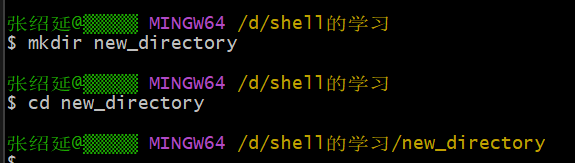
\includegraphics[width=0.5\linewidth]{shell6.png}
  % 图片标题
  \captionof{figure}{创建与切换新目录}
  \label{fig:example}
\end{minipage}

7.函数的创建和使用
\begin{verbatim}
    greet() {
      echo "Hello, $1!"
    }
  
    greet "Shell"
       
\end{verbatim}

\noindent
\begin{minipage}{\linewidth}
 \centering
  % 插入图片
  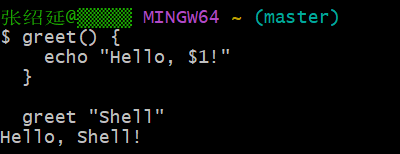
\includegraphics[width=0.5\linewidth]{shell7.png}
  % 图片标题
  \captionof{figure}{定义函数与使用}
  \label{fig:example}
\end{minipage}

8.加法运算
\begin{verbatim}
    a=5
    b=7
    sum=$(($a + $b))
    echo "The sum of $a and$b is: $sum"
\end{verbatim}



\noindent
\begin{minipage}{\linewidth}
 \centering
  % 插入图片
  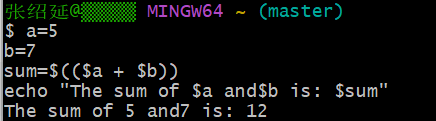
\includegraphics[width=0.5\linewidth]{shell8.png}
  % 图片标题
  \captionof{figure}{进行加法运算}
  \label{fig:example}
\end{minipage}

9. 获取工作目录,并列出工作目录
\begin{verbatim}
    # 获取当前工作目录
    pwd
    # 列出当前目录下的所有文件和目录
    ls -l
\end{verbatim}

\begin{minipage}{\linewidth}
    \centering
     % 插入图片
     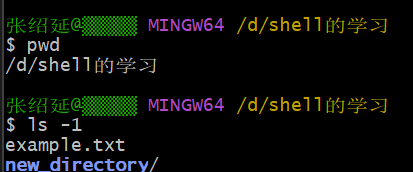
\includegraphics[width=0.5\linewidth]{shell9.png}
     % 图片标题
     \captionof{figure}{获取目录并列出当前目录}
     \label{fig:example}
\end{minipage}


10.查看当前目录文件数目
\begin{verbatim}
    file_count=$(ls -1 | wc -l)
    echo "There are $file_count files in the current directory."
\end{verbatim}


\noindent
\begin{minipage}{\linewidth}
 \centering
  % 插入图片
  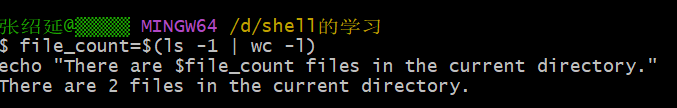
\includegraphics[width=0.5\linewidth]{shell10.png}
  % 图片标题
  \captionof{figure}{查看当前目录文件数目}
  \label{fig:example}
\end{minipage}



\subsection{Vim学习例子10个}
1.Vim文件的创立,
在终端中输入 vim example.txt


\noindent
\begin{minipage}{\linewidth}
  \centering
  % 插入图片
  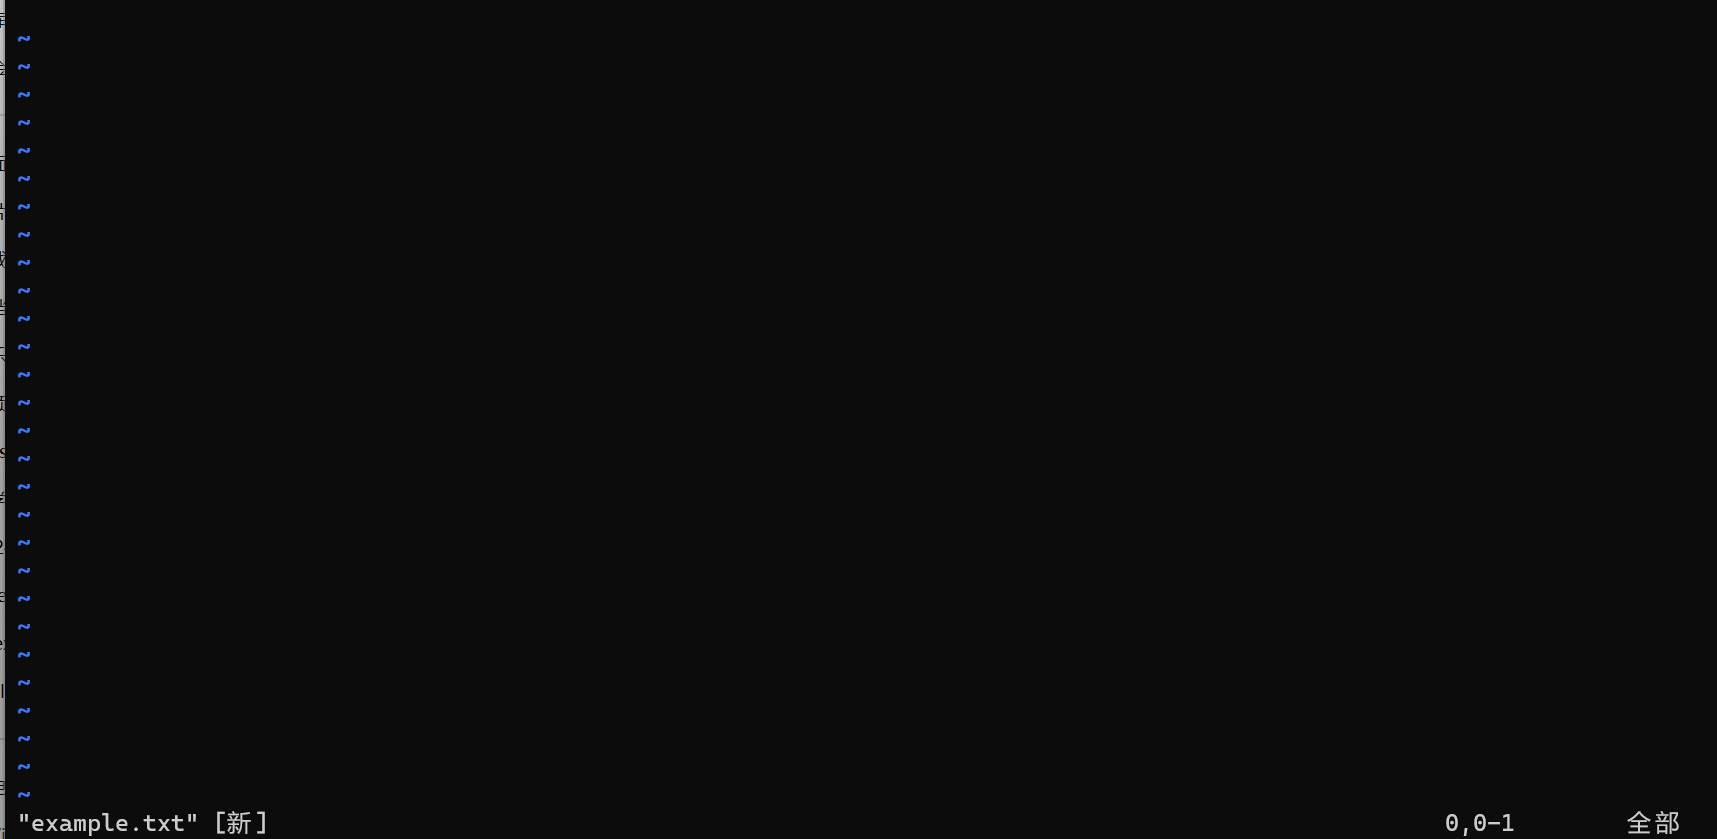
\includegraphics[width=0.5\linewidth]{vim1.png}
  % 图片标题
  \captionof{figure}{Vim文件的创立}
  \label{fig:example}
\end{minipage}

2. i键为插入,开始输入内容hello,vim!

\noindent
\begin{minipage}{\linewidth}
  \centering
  % 插入图片
  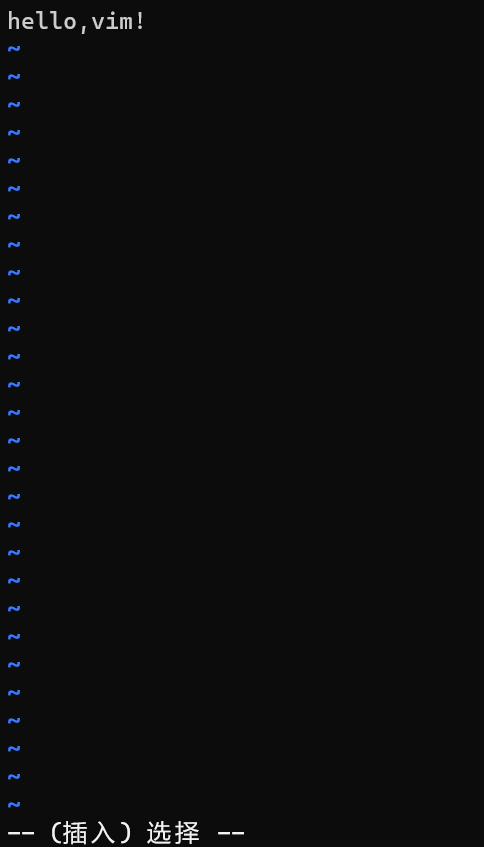
\includegraphics[width=0.5\linewidth]{vim2.png}
  % 图片标题
  \captionof{figure}{i插入内容}
  \label{fig:example}
\end{minipage}

3.编辑的退出与保存
\begin{verbatim}
   Esc是回到正常模式
   :w带编者保存
   :q代表退出
   如果不按w的话则文件为SWP文件,用于临时储存数据
\end{verbatim}

\noindent
\begin{minipage}{\linewidth}
 \centering
  % 插入图片
  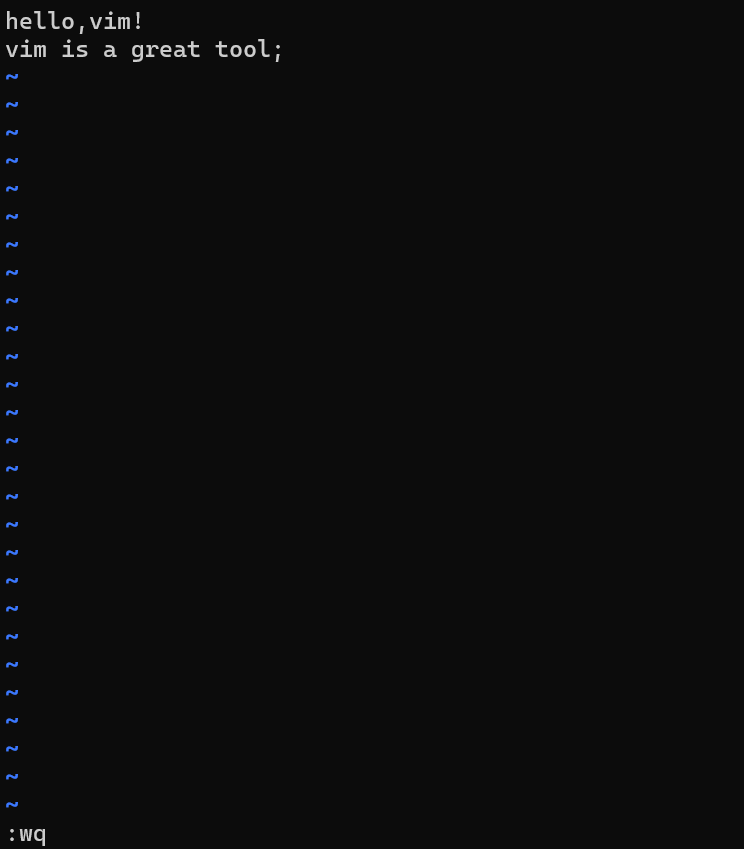
\includegraphics[width=0.5\linewidth]{vim3.png}
  % 图片标题
  \captionof{figure}{编辑的退出与保存}
  \label{fig:example}
\end{minipage}



4.dd表示删除当前行
\begin{verbatim}
   在vim is a greet tool前输入dd删除后的结果
\end{verbatim}


\noindent
\begin{minipage}{\linewidth}
 \centering
  % 插入图片
  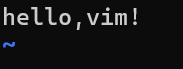
\includegraphics[width=0.5\linewidth]{vim4.png}
  % 图片标题
  \captionof{figure}{dd删除当前行后的结果}
  \label{fig:example}
\end{minipage}

5.dw:删除光标后的单词。

\noindent
\begin{minipage}{\linewidth}
 \centering
  % 插入图片
  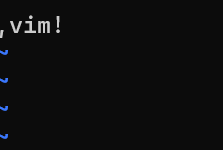
\includegraphics[width=0.5\linewidth]{vim5.png}
  % 图片标题
  \captionof{figure}{dw删除光标后的单词的结果}
  \label{fig:example}
\end{minipage}

6.x:删除光标下的字符。

\noindent
\begin{minipage}{\linewidth}
 \centering
  % 插入图片
  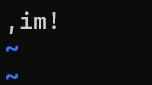
\includegraphics[width=0.5\linewidth]{vim6.png}
  % 图片标题
  \captionof{figure}{删除光标下的字符的结果}
  \label{fig:example}
\end{minipage}

7.r:替换光标下的单个字符。
R:进入替换模式,连续替换多个字符直到按下 Esc。


\noindent
\begin{minipage}{\linewidth}
 \centering
  % 插入图片
  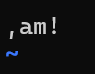
\includegraphics[width=0.5\linewidth]{vim7.png}
  % 图片标题
  \captionof{figure}{用r替换光标下的单个字符}
  \label{fig:example}
\end{minipage}

\noindent
\begin{minipage}{\linewidth}
 \centering
  % 插入图片
  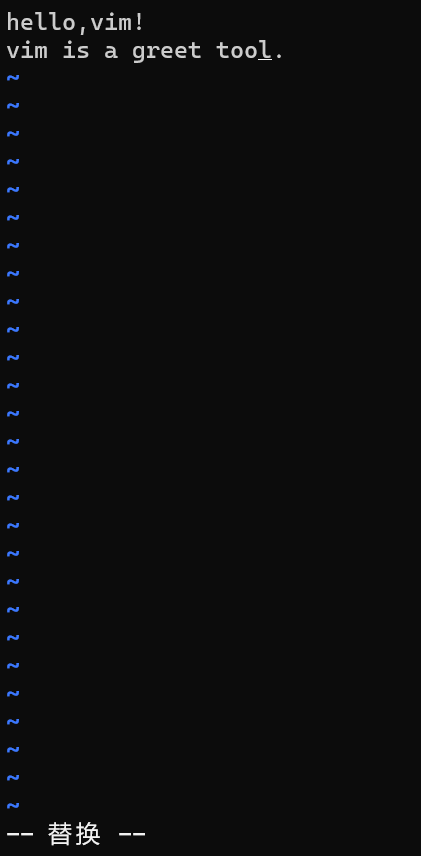
\includegraphics[width=0.5\linewidth]{vim8.png}
  % 图片标题
  \captionof{figure}{在R模式未改变前}
  \label{fig:example}
\end{minipage}

\noindent
\begin{minipage}{\linewidth}
 \centering
  % 插入图片
  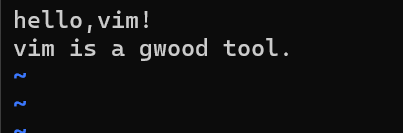
\includegraphics[width=0.5\linewidth]{vim9.png}
  % 图片标题
  \captionof{figure}{在R模式改变后}
  \label{fig:example}
\end{minipage}

8. 
u:撤销最后一次更改。

Ctrl + r:重做最后一次撤销,即反撤销。


\begin{minipage}{\linewidth}
    \centering
     % 插入图片
     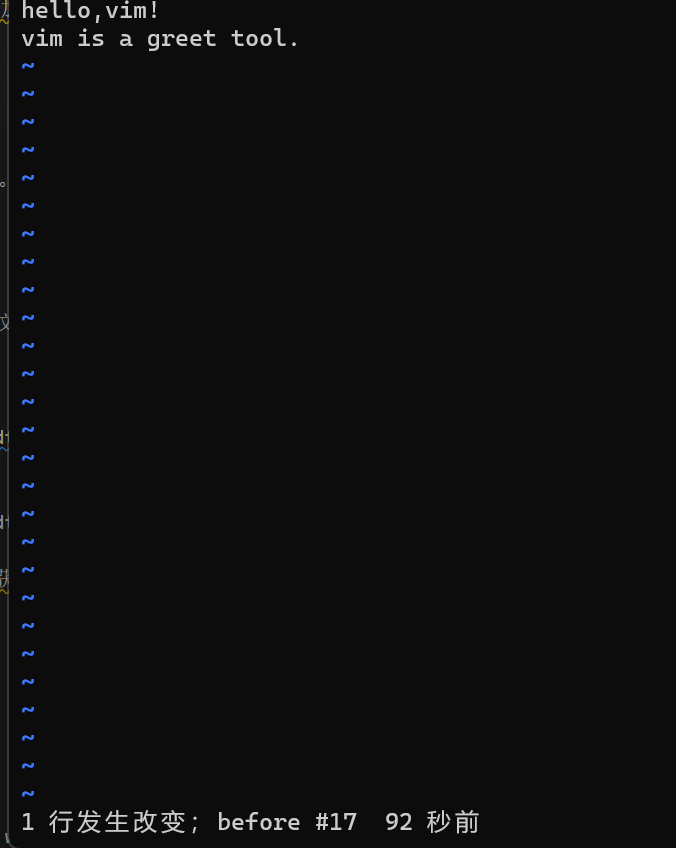
\includegraphics[width=0.5\linewidth]{vim10.png}
     % 图片标题
     \captionof{figure}{撤销}
     \label{fig:example}
\end{minipage}

\begin{minipage}{\linewidth}
  \centering
   % 插入图片
   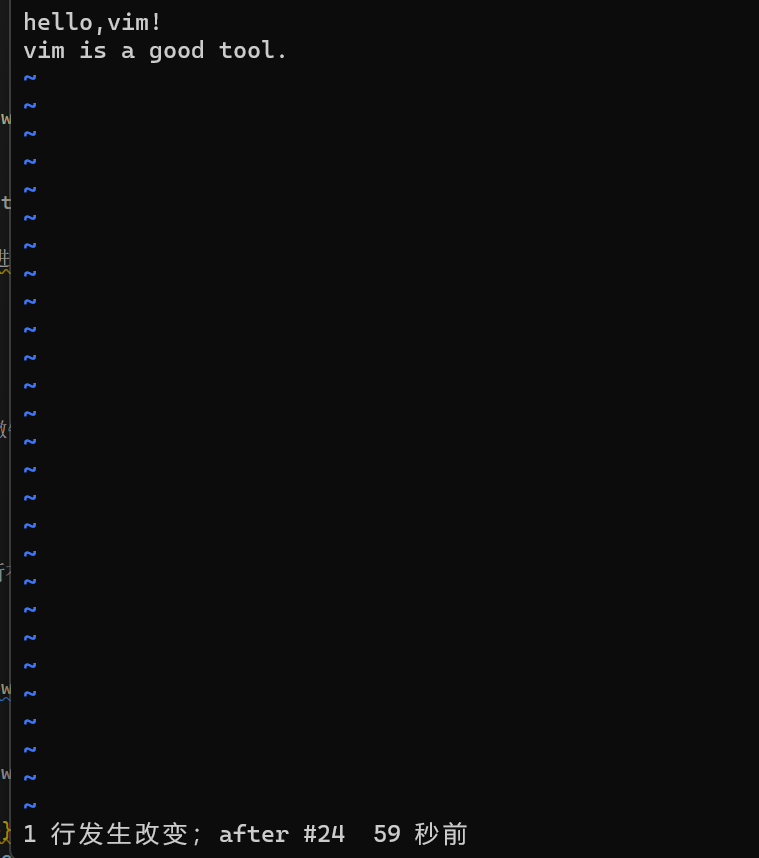
\includegraphics[width=0.5\linewidth]{vim11.png}
   % 图片标题
   \captionof{figure}{反撤销}
   \label{fig:example}
\end{minipage}


9.复制的学习:

复制单行:
将光标移动到要复制的行的任意位置。
输入 yy 来复制整行。

复制部分行:
将光标移动到要开始复制的位置。
进入可视化模式,可以按 v(用于字符模式)或 V(用于行模式)。
使用光标键hjkl选择要复制的文本。
一旦选择了文本,按 y 来复制选中的文本。

复制多个行:
将光标移动到要复制的第一行的任意位置。
输入 数字yy,其中 “数字” 是您想要复制的行数。
例如,3yy 会复制光标所在的当前行以及下面两行,总共三行。

\noindent
\begin{minipage}{\linewidth}
 \centering
  % 插入图片
  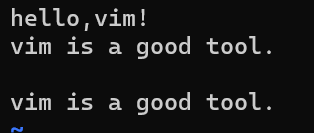
\includegraphics[width=0.5\linewidth]{vim12.png}
  % 图片标题
  \captionof{figure}{复制一行后的结果}
  \label{fig:example}
\end{minipage}

\noindent
\begin{minipage}{\linewidth}
 \centering
  % 插入图片
  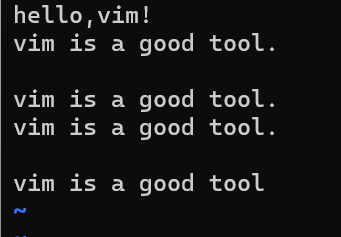
\includegraphics[width=0.5\linewidth]{vim13.png}
  % 图片标题
  \captionof{figure}{选择性复制后的结果}
  \label{fig:example}
\end{minipage}


10.
p:在光标后粘贴。
P:在光标前粘贴。
下面是粘贴后的结果

\noindent
\begin{minipage}{\linewidth}
 \centering
  % 插入图片
  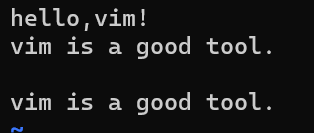
\includegraphics[width=0.5\linewidth]{vim12.png}
  % 图片标题
  \captionof{figure}{粘贴后的结果}
  \label{fig:example}
\end{minipage}




\section{解题感悟}
Shell是一种强大的自动化工具。通过编写脚本,可以将日常繁琐的任务变得简单高效,这让我对编程产生了浓厚的兴趣,也锻炼了我的逻辑思维能力。
与此同时,Shell的学习让我更加深入地理解了操作系统的内部工作原理,我开始意识到,每一个命令背后都隐藏着复杂而精巧的设计,这激发了我对技术的探索欲。

Vim完全改变了我对文本编辑的看法。起初,Vim的模式系统和快捷键让我感到困惑,但随着时间的推移,熟练使用Vim后,我编辑文本的速度和准确性都有了显著提升。
Vim的学习过程也是对个人习惯的一次挑战。它要求我放弃一些固有的操作习惯,转而接受一种更高效的工作方式。这个过程虽然艰难,但也让我认识到,改变习惯需要时间和耐心,而一旦新的习惯形成,它将带来巨大的收益。

总的来说,Shell和Vim的学习不仅仅提升了我的技术能力,更让我在解决问题的思维方式上有了新的认识。

github路径
您可以在此查看项目的源代码: 

\url{https://github.com/AmbitiousLight/AmbitiousLight/tree/ff751aec5aaa0eb9b01d6326244bc747e2921e2b/Latex%E8%AE%BA%E6%96%87}
\end{document}
